\documentclass[12pt,a4paper]{report}

\usepackage[utf8x]{inputenc}
\usepackage{amsmath}
\usepackage{amsfonts}
\usepackage{amssymb}
\usepackage{graphicx}
\usepackage{enumitem}
\usepackage{fontspec}
\usepackage{pgf}
\usepackage{tikz}
\usepackage{calrsfs}
\usepackage{ifthen}
\usepackage{algpseudocode}
%\usepackage[linesnumbered,lined,boxed,commentsnumbered]{algorithm2e}
\usetikzlibrary{graphs, shapes, snakes, graphdrawing}
\usegdlibrary{layered, force}

\begin{document}

\begin{titlepage}
	\centering
	{\scshape\LARGE Universidad Nacional Autónoma de México \par}
	\vspace{1cm}
	{\scshape\Large Computación Distribuida\par}
	\vspace{1.5cm}
	{\huge\bfseries Tarea 3\par}
	\vspace{.5cm}
	{\Large\itshape Edgar Quiroz Castañeda \par}
    \vspace{.5cm}
	{\Large\itshape Jerónimo Almeida Rodríguez \par}
	\vfill
	 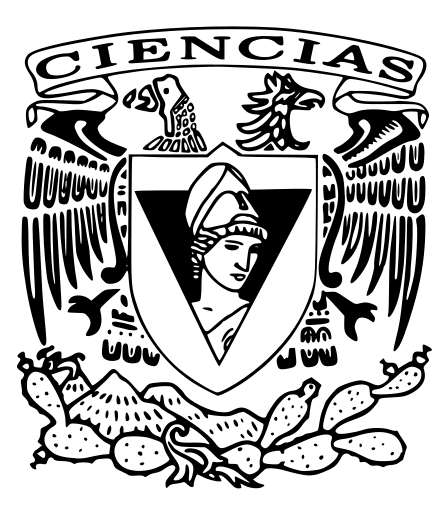
\includegraphics[width=0.5\textwidth]{escudo_f-ciencias.png}
	\vfill

% Bottom of the page
	{\large Jueves 30 de Agosto del 2018 \par}
\end{titlepage}

\pagebreak
\setlength{\voffset}{-0.75in}
\setlength{\headsep}{5pt}

%\newcommand{\ed}[2]{(#1) edge (#2)}
%\newcommand{\eee}[4]{\path [->,draw,thin] ($ (#1) !.5! (#2)$) -- ($ (#3) !.5! (#4) $);}


\begin{enumerate}
	%Ejercicio 1
	\item {
		Dados los procesos $A$ y $B$, diseña un algoritmo para el ataque coordinado
		proximado (aproximate agreement) en el que para llegar al acuerdo deben decidir
		valores que estén a distancia a lo más $\frac{1}{2^k}$ y utilice menos rondas
		de comunicación que el algoritmo visto en clase.\\

		Notemos que utilizando el algoritmo visto en clase, pasa que si en alguna
		ronda los dos procesos tienen el mismo valor, entonces tendrán ese mismo
		valor por todas las rondas restantes.\\

		El algoritmo propuesto es el siguiente:\\

		\begin{algorithmic}[1]
					\Require $init \in \{0, 1\}$
					\Function{$\frac{1}{3}-AproximateAgreement$}{$init$}
						\State $send(init)$
						\State $x \gets receive()$
						\If{$x \ne null$}
							\State \Return $\frac{init + 2x}{3}$
						\Else
							\State \Return $init$
						\EndIf
					\EndFunction
				\end{algorithmic}
	}

	%Ejercicio 2
	\item {
		Dibuja la gráfica del protocolo que diseñaste para 2 rondas para $k = 2$.
		Para cada vértice indica el valor de salida y para cada arista indica el
		patrón de mensajes recibidos.\\\\

		\begin{tikzpicture}[scale = 1.4]
			\tikzstyle{every node} = [draw, shape = circle]
			\foreach \i/\s in {0/$A \longrightarrow B$, 6/$A\longleftarrow B$}{
				\node at (\i, 9) (Bu\i) [label = above : {1}] {$B$};
				\node at (\i + 3, 9) (Au\i) [label = above : {1}] {$A$};
				\ifthenelse{\i = 6}{\draw (Au0) -- node[rectangle,above,draw=none]{$A\longleftrightarrow B$}++(Bu\i);}{}
				\draw (Au\i) --node[rectangle, above, draw=none, label = above : {\s}]{\s}++ (Bu\i) ;
				\node at (\i, 0) (Al\i) [label = below : {0}] {$A$};
				\node at (\i + 3, 0) (Bl\i) [label = below : {0}] {$B$};
				\ifthenelse{\i = 6}{\draw (Bl0) -- node[rectangle, below, draw=none]{$A\longleftrightarrow B$}++ (Al\i);}{}
				\draw (Al\i) --node[rectangle, below, draw=none, label = below : {\s}]{\s}++ (Bl\i);
			}
			\foreach \i/\j/\k/\s/\c in {2/0/3, 4/2/2, 6/4/2, 8/6/1}{
				\node at (0, \i) (Ai\i) [label = left : {\k/4}] {$A$};
				\node at (0, \i - 1) (Bi\i) [label = left : {\k/4}] {$B$};
				\ifthenelse{\i > 2}{\draw (Ai\j) -- (Bi\i);}{}
				\draw (Ai\i) -- (Bi\i);
				\node at (9, \i - 1) (Ad\i) [label = right : {\k/4}] {$A$};
				\node at (9, \i) (Bd\i) [label = right : {\k/4}] {$B$};
				\ifthenelse{\i > 2}{\draw (Bd\j) -- (Ad\i);}{}
				\draw (Ad\i) -- (Bd\i);
			}
		\end{tikzpicture}
	}


\end{enumerate}
\end{document}
